\section{Задание}
По выданному преподавателем варианту восстановить текст заданного варианта программы, определить предназначение и составить описание программы, определить область представления и область допустимых значений исходных данных и результата, выполнить трассировку программы.
\begin{figure}[H]
\centering
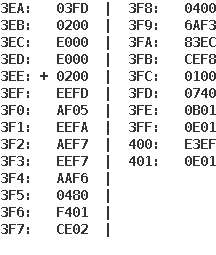
\includegraphics[scale=0.6]{task}
\label{pic:task}
\end{figure}

\section{Текст программы}
\begin{center}
\begin{tabular}{|c|c|c|l|}
\hline
\textbf{Адрес ячейки} & \textbf{Содержимое ячейки} & \textbf{Мнемоника} & \textbf{Комментарии}\\
\hline
58B & 05A1 & --- & Адрес начала массива\\
58C & 0200 & --- & Ячейка для хранения адреса \\
 & & & обрабатываемого элемента массива\\
58D & E000 & --- & Ячейка для хранения количества \\
 & & &необработанных элементов массива\\
58E & 0200 & --- & Ячейка для записи результата  \\ 
& & & работы программы\\
\hline
\hline
58F & 0200 & CLA & Очистка аккумулятора\\
590 & EEFD & ST (IP $-$ 3) & Сохраняем аккумулятор в ячейку 0x58E\\
\hline
591 & AF05 & LD \#0x5 & Загружаем в AC \#0x5\\
592 & EEFA & ST (IP $-$ 6) & Сохраняем AC в 0x58D\\
\hline
593 & 4EF7 & ADD (IP $-$ 9) & Складываем AC с элементом в 0x58B\\
594 & EEF7 & ST (IP $-$ 9) & Сохраняем AC в ячейку 0x58C\\
\hline
595 & ABF6 & LD $-$ (IP $-$ 10) & Загружаем элемент массива по адресу в \\
 & & & ячейке 0x58C (предекрементировав)\\
596 & F202 & BMI (IP $+$ 2) & Если N==1, то IP -> 599\\
597 & 0300 & CLC & Очистка бита переноса C\\
598 & 0380 & CMC & Инверсия бита переноса C\\
599 & 0200 & CLA & Очистка аккумулятора\\
59A & 0280 & NOT & Инверсия битов переноса аккумулятора\\
59B & 2EF2 & AND (IP $-$ 14) & AC \& 0x58E -> AC\\
59C & 0400 & ROL & Цикличиский сдвиг влево\\
59D & EEF0 & ST (IP $-$ 16) & Сохраняем результат в ячейку 0x58E\\
59E & 858D & LOOP 0x58D & Если $MEM(0x58D)\leq 0$ то IP + 1 -> IP\\
59F & CEF5 & BR (IP $-$ 11) & Безусловный переход в ячейку 0x595\\
5A0 & 0100 & HLT & Отключение тактового генератора\\
\hline
\hline
5A1 & 759B & --- & \\
5A2 & 0500 & --- & \\
5A3 & F400 & --- & Элементы массива\\
5A4 & 0280 & --- & \\
5A5 & 459E & --- & \\
\hline
\end{tabular}
\end{center}

\newpage


\section{Описание программы}
\subsection{Назначение программа и реализуемая ею формула}
Программа проходит каждый элемент массива с конца и исследует его элементы на знак (положительные/отрицательные). Если элемент отрицательный, то в результат записывается 0, если же положительный или больше нуля, то 1.

\begin{center}
	\textit{Реализуемая формула}
	\[ D (0x58E) = \sum_{i=1}^{5} \textrm{ if (array[i] \geq 0) $2^{5-i}$ else 0}\]
\end{center}

\subsection{Область представления и область допустимых значений исходных данных и результата}
\subsubsection{Область представления}
\noindent Ячейки 5A1--5A5: 16-разрядные знаковые целые числа, с фиксированной запятой. Диапазон значений формата: $-2^{15}\ldots2^{15}-1$\\
\\
Ячейки 58B: 11-разрядное беззнаковое целое число, с фиксированной запятой. Диапазон значений формата: $0\ldots2^{11} - 1$\\
\\
Ячейка 58E: 16-разрядное беззнаковое целое число, с фиксированной запятой. Диапазон значений формата: $0\ldots2^{16} - 1$\\


\subsubsection{Область допустимых значений}
\noindent Область допустимых значений ячеек 5A1--5A5 совпадает с областью их представления.\\
\\
Областью допустимых значений ячейки 58B - ячейки, хранящей адрес начала массива, будет являться промежуток $[000, 586]\cup[5A1,7FF]$\\
\\
Область допустимых значений ячейки 58E совпадает с областью ее представления.\\

\subsection{Расположение в памяти программы, исходных данных и результатов}
\noindent 	B (0x58B) - aдрес начала массива\\
R (0x58E) - ячейка для записи результата работы программы\\
Ячейки 58C, 58D - вспомогательные ячейки для хранения данных, нужных для функционирования программы\\
Ячейки 58F--5A0 - код программы\\

\subsection{Адреса первой и последней выполняемой команд программы}
\noindent Ячейка 58F - первая исполняемая команда\\
Ячейка 5A0 - последняя исполняемая команда\\

\newpage
\section{Таблица трассировки}
\resizebox{16cm}{!}{
\begin{center}
	\begin{tabular}{|c|c|c|c|c|c|c|c|c|c|c|c|}
		\hline
		\multicolumn{2}{|c}{\makecell{\textbf{Выполняемая}\\\textbf{команда}}}
		&\multicolumn{8}{|c|}{\textbf{Содердимое регистров после выполнения команды}}
		&\multicolumn{2}{c|}{\makecell{\textbf{Ячейка, содержимое}\\\textbf{которой изменилось}}}\\
		\hline
		Адрес & Код & IP & CR & AR & DR & SP & BR & AC & NZVC & Адрес & Новый код\\
		\hline
		58F & 0200 & 590 & 0200 & 58F & 0200 & 000 & 058F & 0000 & 0100 & --- & ---\\
		\hline
		590 & EEFD & 591 & EEFD & 58E & 0000 & 000 & FFFD & 0000 & 0100 & 58E & 0000\\
		\hline
		591 & AF05 & 592 & AF05 & 591 & 0005 & 000 & 0005 & 0005 & 0000 & --- & ---\\
		\hline
		592 & EEFA & 593 & EEFA & 58D & 0005 & 000 & FFFA & 0005 & 0000 & 58D & 0005\\
		\hline
		593 & 4EF7 & 594 & 4EF7 & 58B & 05A1 & 000 & FFF7 & 05A6 & 0000 & --- & ---\\
		\hline
		594 & EEF7 & 595 & EEF7 & 58C & 05A6 & 000 & FFF7 & 05A6 & 0000 & 58C & 05A6\\
		\hline
		595 & ABF6 & 596 & ABF6 & 5A5 & 459E & 000 & FFF6 & 459E & 0000 & 58C & 05A5\\
		\hline
		596 & F202 & 597 & F202 & 596 & F202 & 000 & 0596 & 459E & 0000 & --- & ---\\
		\hline
		597 & 0300 & 598 & 0300 & 597 & 0300 & 000 & 0597 & 459E & 0000 & --- & ---\\
		\hline
		598 & 0380 & 599 & 0380 & 598 & 0380 & 000 & 0598 & 459E & 0001 & --- & ---\\
		\hline
		599 & 0200 & 59A & 0200 & 599 & 0200 & 000 & 0599 & 0000 & 0101 & --- & ---\\
		\hline
		59A & 0280 & 59B & 0280 & 59A & 0280 & 000 & 059A & FFFF & 1001 & --- & ---\\
		\hline
		59B & 2EF2 & 59C & 2EF2 & 58E & 0000 & 000 & FFF2 & 0000 & 0101 & --- & ---\\
		\hline
		59C & 0400 & 59D & 0400 & 59C & 0400 & 000 & 059C & 0001 & 0000 & --- & ---\\
		\hline
		59D & EEF0 & 59E & EEF0 & 58E & 0001 & 000 & FFF0 & 0001 & 0000 & 58E & 0001\\
		\hline
		59E & 858D & 59F & 858D & 58D & 0003 & 000 & 059E & 0001 & 0000 & 58D & 0004\\
		\hline
		59F & CEF5 & 595 & CEF5 & 59F & 595 & 000 & FFF5 & 0001 & 0000 & --- & ---\\
		\hline
		595 & ABF6 & 596 & ABF6 & 5A4 & 0280 & 000 & FFF6 & 0280 & 0000 & 58C & 05A4\\
		\hline
		596 & F202 & 597 & F202 & 596 & F202 & 000 & 0596 & 0280 & 0000 & --- & ---\\
		\hline
		597 & 0300 & 598 & 0300 & 597 & 0300 & 000 & 0597 & 0280 & 0000 & --- & ---\\
		\hline
		598 & 0380 & 599 & 0380 & 598 & 0380 & 000 & 0598 & 0280 & 0001 & --- & ---\\
		\hline
		599 & 0200 & 59A & 0200 & 599 & 0200 & 000 & 0599 & 0000 & 0101 & --- & ---\\
		\hline
		59A & 0280 & 59B & 0280 & 59A & 0280 & 000 & 059A & FFFF & 1001 & --- & ---\\
		\hline
		59B & 2EF2 & 59C & 2EF2 & 58E & 0001 & 000 & FFF2 & 0001 & 0001 & --- & ---\\
		\hline
		59C & 0400 & 59D & 0400 & 59C & 0400 & 000 & 059C & 0003 & 0000 & --- & ---\\
		\hline
		59D & EEF0 & 59E & EEF0 & 58E & 0003 & 000 & FFF0 & 0003 & 0000 & 58E & 0003\\
		\hline
		59E & 858D & 59F & 858D & 58D & 0002 & 000 & 059E & 0003 & 0000 & 58D & 0003\\
		\hline
		59F & CEF5 & 595 & CEF5 & 59F & 595 & 000 & FFF5 & 0003 & 0000 & --- & ---\\
		\hline
		595 & ABF6 & 596 & ABF6 & 5A3 & F400 & 000 & FFF6 & F400 & 1000 & 58C & 05A3\\
		\hline
		596 & F202 & 599 & F202 & 596 & F202 & 000 & 0002 & F400 & 1000 & --- & ---\\
		\hline
		599 & 0200 & 59A & 0200 & 599 & 0200 & 000 & 0599 & 0000 & 0100 & --- & ---\\
		\hline
		59A & 0280 & 59B & 0280 & 59A & 0280 & 000 & 059A & FFFF & 1000 & --- & ---\\
		\hline
		59B & 2EF2 & 59C & 2EF2 & 58E & 0003  & 000 & FFF2 & 0003 & 0000 & --- & ---\\
		\hline
		59C & 0400 & 59D & 0400 & 59C & 0400 & 000 & 059C & 0006 & 0000 & --- & ---\\
		\hline
		59D & EEF0 & 59E & EEF0 & 58E & 0006 & 000 & FFF0 & 0006 & 0000 & 58E & 0006\\
		\hline
		59E & 858D & 59F & 858D & 58D & 0001 & 000 & 059E & 0006 & 0000 & 58D & 0002\\
		\hline
		59F & CEF5 & 595 & CEF5 & 59F & 595 & 000 & FFF5 & 0006 & 0000 & --- & ---\\
		\hline
		595 & ABF6 & 596 & ABF6 & 5A2 & 0500 & 000 & FFF6 & 0500 & 0000 & 58C & 05A2\\
		\hline
		596 & F202 & 597 & F202 & 596 & F202 & 000 & 0596 & 0500 & 0000 & --- & ---\\
		\hline
		597 & 0300 & 598 & 0300 & 597 & 0300 & 000 & 0597 & 0500 & 0000 & --- & ---\\
		\hline
		598 & 0380 & 599 & 0380 & 598 & 0380 & 000 & 0598 & 0500 & 0001 & --- & ---\\
		\hline
		599 & 0200 & 59A & 0200 & 599 & 0200 & 000 & 0599 & 0000 & 0101 & --- & ---\\
		\hline
		59A & 0280 & 59B & 0280 & 59A & 0280 & 000 & 059A & FFFF & 1001 & --- & ---\\
		\hline
		59B & 2EF2 & 59C & 2EF2 & 58E & 0006 & 000 & FFF2 & 0006 & 0001 & --- & ---\\
		\hline
		59C & 0400 & 59D & 0400 & 59C & 0400 & 000 & 059C & 000D & 0000 & --- & ---\\
		\hline
		59D & EEF0 & 59E & EEF0 & 58E & 000D & 000 & FFF0 & 000D & 0000 & 58E & 000D\\
		\hline
		59E & 858D & 59E & 858D & 58D & 0000 & 000 & 059E & 000D & 0000 & 58D & 0001\\
		\hline
		59F & CEF5 & 595 & CEF5 & 59F & 595 & 000 & FFF5 & 000D & 0000 & --- & ---\\
		\hline
		595 & ABF6 & 596 & ABF6 & 5A1 & 759B & 000 & FFF6 & 759B & 0000 & 58C & 05A1\\
		\hline
		596 & F202 & 597 & F202 & 596 & F202 & 000 & 0596 & 759B & 0000 & --- & ---\\
		\hline
		597 & 0300 & 598 & 0300 & 597 & 0300 & 000 & 0597 & 759B & 0000 & --- & ---\\
		\hline
		598 & 0380 & 599 & 0380 & 598 & 0380 & 000 & 0598 & 759B & 0001 & --- & ---\\
		\hline
		599 & 0200 & 59A & 0200 & 599 & 0200 & 000 & 0599 & 0000 & 0101 & --- & ---\\
		\hline
		59A & 0280 & 59B & 0280 & 59A & 0280 & 000 & 059A & FFFF & 1001 & --- & ---\\
		\hline
		59B & 2EF2 & 59C & 2EF2 & 58E & 000D & 000 & FFF2 & 000D & 0001 & --- & ---\\
		\hline
		59C & 0400 & 59D & 0400 & 59C & 0400 & 000 & 059C & 001B & 0000 & --- & ---\\
		\hline
		59D & EEF0 & 59E & EEF0 & 58E & 001B & 000 & FFF0 & 001B & 0000 & 58E & 001B\\
		\hline
		59E & 858D & 5A0 & 858D & 58D & FFFF & 000 & 059E & 001B & 0000 & 58D & 0000\\
		\hline
		5A0 & 0100 & 5A1 & 0100 & 5A0 & 0100 & 000 & 5A0 & 001B & 0000 & --- & ---\\
		\hline
	\end{tabular}
\end{center}

}

\section{Вывод}
В ходе выполнения данной лабораторной работы я познакомился с режимами адресации БЭВМ. Также потрогал новые для меня команды - команды ветвления, сравнения, команду LOOP. На практике разобрался с циклом выборки адреса для разных режимов адресации.